\section{Sensoren}
\label{sec:sensor}

Zur Detektion von Kot oder Urin steht eine Vielzahl an Sensoren zur
Verfügung. Eine Auswahl derer wären: Gas, Temperatur, Feuchtigkeit,
Gewicht, Luftfeuchtigkeit, uvm. Die Auswahl verringert sich durch
einige ergonomische und medizinische und technische Anforderungen, wie
zum Beispiel Hautverträglichkeit, Wasserfestigkeit, Langlebigkeit,
Größe und Waschbarkeit. Durch diese Spezifikationen fielen zum
Beispiel Gas, Luftfeuchtigkeit aus der Auswahl, da Diese nicht
wasserfest sind und somit nicht in der Windel zum Einsatz kommen
können. Ein Gewichts- bzw Drucksensor  konnte nicht verwendet werden,
da das Aufsetzen/Hinsetzen des Babys zum Auslösen führen würde.
Nach Ausschluss vieler möglicher Detektionsverfahren, wurde in diesem
Projekt das Hauptziel auf die Konstruktion und den Entwurf eines
Feuchtigkeitssensors, welcher in Zusammenarbeit mit einem
Temperatursensor die Ausscheidung eines Babys erkennt und in Folge
dessen ein Signal versendet, wie es im Kapitel „Kommunikation“ näher
beschrieben wird gelegt. Um ein Fehlauslösen und somit einen Fehlalarm
zu vermeiden, wurden die Sensoren miteinander verknüpft und nur ein
Auslösen Beider führt zur Sendung eines Trigger Signals.
Im Folgenden werden die verwendeten Sensoren, sowie deren
Funktionsweise näher erläutert.


\subsection{Temperatursensor}
Da die Ausscheidungen eines Menschen die Körperkerntemperatur besitzen
und diese um einige Grad höher ist als die Oberflächentemperatur, kann
dieser Unterschied leicht detektiert werden und als Signal verwendet
werden. Die anfängliche Idee eine Temperaturschwelle festzulegen und
bei Überschreitung Dieser ein Signal auszulösen, wurde verworfen da
das Ansteigen der Umgebungstemperatur oder ein Fieber zum Anschlagen
des Sensors führen würde und somit einen Fehlalarm auslösen könnte.
Diese Änderungen entstehen über einen längeren Zeitraum, wohingegen
das Ausscheiden von Exkrementen in kurzer Zeit stattfindet. Die daraus
resultierende schnelle Veränderung lässt sich einfach detektieren und
deutet mit sehr hoher Wahrscheinlichkeit auf Exkretion hin.
Die erste Version des Sensors wurde mittels einer Wheatstone-Brücke
realisiert. Diese Schaltung ist eine Widerstandsbrücke, welche aus
zwei parallelgeschalteten Spannungsteilern mit identischen
Widerständen besteht. Mindestens einer dieser Widerstände wird als PTC
oder NTC realisiert. Bei einer abgeglichenen Brückenschaltung ist das
Potenzial zwischen den Mittelpunkten der Spannungsteiler Null. Sobald
sich also ein Widerstand ändert, ändert sich auch der
Potenzialunterschied. Ein großer Vorteil dieser Messbrücke ist die
Genauigkeit der Messung, welche ohne Offset vorliegt. Jedoch ist
dieser Vorteil in diesem Projekt ein großer Nachteil, da die Schaltung
sehr sensibel ist. Außerdem ist das Abgleichen quasi unmöglich durch
die unterschiedlichen Körpertemperaturen bzw. Außentemperaturen. 
Aufgrund dieses Nachteils und der nicht vorhandenen Notwendigkeit der
Genauigkeit, wurde sich gegen eine Wheatstone-Brücke entschieden.

\begin{figure}
\centering
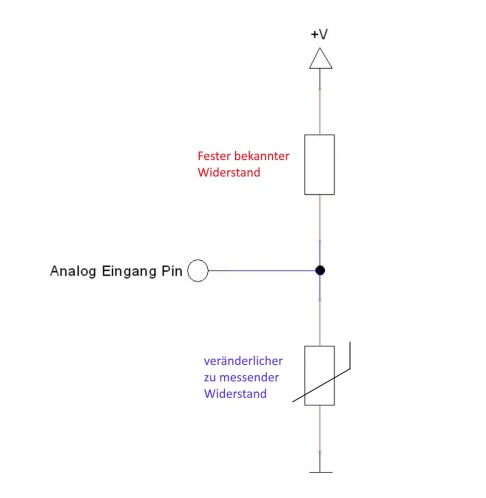
\includegraphics[width=.6\textwidth]{includes/sensor_pics/486px-KY-013_VoltDivide.jpg}
\caption{Aufbau der Sensorschaltung}
\label{fig:tempsens}
\end{figure}

Die zweite Version des Sensors wurde mittels eines analogen
Temperatursensors (KY-013) realisiert, welcher im Arduino Sensor kit
vorhanden ist. Dieses Modul besteht aus einem festen Widerstand als
Referenz und zur Strombegrenzung in Reihe mit einem
temperaturveränderlichen NTC-Thermistor (Bild \ref{fig:tempsens}),
welcher mit steigender Temperatur einen geringer werdenden Widerstand
hat (Bild \ref{fig:tempkurve}).

\begin{figure}
\centering
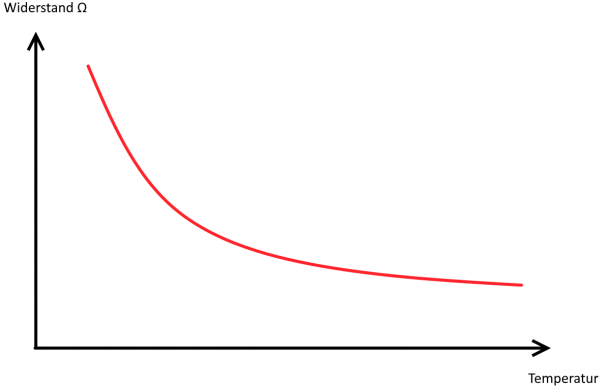
\includegraphics[width=.6\textwidth]{includes/sensor_pics/610px-KY-013_NTC-Kurve.png}
\caption{Änderung des Widerstands mit steigender
Temperatur.}
\label{fig:tempkurve}
\end{figure}

``Diese Änderung des Widerstands lässt sich mathematisch annähern und
in einen linearen Verlauf umrechnen und den Temperaturkoeffizienten
(Abhängigkeit von Widerstandsänderung zur Temperaturänderung)
bestimmen. Mittels diesen lässt sich somit dann immer die aktuelle
Temperatur errechnen, wenn man den aktuellen Widerstand kennt. Dieser
Widerstand lässt sich mit Hilfe eines Spannungsteilers bestimmen, wo
sich eine bekannte Spannung über den bekannten und den unbekannten
(veränderlichen) Widerstand aufteilt. Mittels dieser gemessenen
Spannung lässt sich dann der Widerstand berechnen - die genaue
Berechnung ist in dem unten stehenden Codezeilen
enthalten.''\footnote{Text und Bilder entnommen von:
\url{http://sensorkit.joy-it.net/index.php?title=KY-013_Temperatur-Sensor_Modul}.}

\begin{lstlisting}[language=C, caption=Umrechnung des Analogwerts in Temperatur.]
/* Calculate Temperature from incomming Values */
double Thermistor(int RawADC) {
   double Temp;
   Temp = log(10000.0 * ((1024.0/RawADC - 1)));
   Temp = 1/(0.001129148 + (0.000234125 + (0.0000000876741*Temp*Temp))*Temp);
   Temp = Temp - 273.15;            // Convert Kelvin to Celcius
   //Temp = (Temp * 9.0)/ 5.0 + 32.0; // Convert Celcius to Fahrenheit
   return Temp;
}
\end{lstlisting}

\begin{lstlisting}[language=C, caption=Trigger für Exkretion durch
Temperaturvergleich.]
bool tempSensor (){
   bool returnValueTemp = false;
    
   int readVal = analogRead(sensorPinTemp);
   double temp =  Thermistor(readVal);
	
   difftemp = readVal - oldtemp;
   if (oldtemp != 0 && difftemp > 30) {
      returnValueTemp = true;
   }
   oldtemp = readVal;
   //Serial.println(temp);  // display tempature
   //Serial.println(readVal);  // display tempature
			  
   return returnValueTemp;
}
\end{lstlisting}

Wie im Code zu sehen ist, wurde er so umgeschrieben, dass er auf eine
schnelle Änderung der Temperatur anspricht, was wie oben beschrieben
auf Exkretion hindeutet\footnote{Der komplette Code ist auf
\url{https://github.com/jomaway/poop-face-detection_sensor}.}.
Im Gegensatz zum Feuchtigkeitssensor, welcher flächendeckend in die
Einlage eingenäht ist, misst der Temperatursensor sehr punktuell. Dies
stellt ein Problem dar, da je nach Geschlecht des Babys der Urin an
einer anderen Stelle ausgeschieden wird. Bei Mädchen eher zentral und
bei Jungen etwas weiter nach vorne versetzt. Eine Lösung wäre es, zwei
verschiedene, geschlechtsspezifische Modelle der Einlage anzufertigen.
Eine andere Lösung wäre es, zwei Sensoren zu verwenden, um an beiden
Stellen detektieren zu können, was aber die Kosten des Produkts
steigern würde. Ein nicht praktikabler Lösungsweg wäre eine mittige
Anbringung des Sensors. Die Flüssigkeit würde sich zwar im Stoff bis
dorthin ausbreiten, jedoch wäre die Temperatur bis dort so weit
abgekühlt, dass eine sichere Detektion nicht mehr sichergestellt
werden kann.
Das verwendete Modul ist durch seine rechteckige Form nur für einen
Prototype geeignet. Für die weitere Entwicklung bzw. Verwendung des
Poop-Face-Detection Systems würde ein anderer Sensor, wie ein TMP36
oder Ähnliche mehr Sinn machen, da die Form wesentlich ergonomischer
ist und dieser auch einfach anzuschließen und anzusteuern ist.